\documentclass{article}
%\usepackage[spanish,activeacute]{babel}
%\usepackage[english,activeacute]{babel}
%\usepackage[latin1]{inputenc}
\usepackage[utf8]{inputenc}
\usepackage[english]{babel}

\usepackage{amsmath,amsfonts,amssymb,amstext,amsthm,amscd}
\usepackage{hyperref}
\usepackage{latexsym}
\usepackage{graphicx}
%\usepackage{subfigure}
\usepackage{subfig}
%\linespread{1.6}
\usepackage{float}
\usepackage{dcolumn}% Align table columns on decimal point(esto lo saque del ejemplo de revtex4)
\usepackage{bm}% bold math(esto lo saque del ejemplo de revtex4)
\newcounter{itemR}
\usepackage{here} %recordar usar el comando[H] para las gráficas que es el comando here en lugar de [h!]
\usepackage{fancyhdr}
%\usepackage{sidecap}
%\usepackage[spanish,activeacute]{babel}
\usepackage{multirow}
\usepackage{multicol}
\usepackage{array}
\usepackage{enumitem}
%\usepackage{booktabs}% para hacer tablas profesionales con \toprule

% ------------------------------------------------------------------------------------------------------------------------------------------------------

\usepackage{fancyhdr}
\setlength{\headheight}{15.2pt}
\usepackage[paperwidth=8.5in, paperheight=11.0in, top=1.0in, bottom=1.0in, left=1.0in, right=1.0in]{geometry}

\pagestyle{fancyplain}
\fancyhead[LE,RO]{Práctica $\#$10}
\fancyhead[CE,CO]{}
\fancyhead[RE,LO]{P23-FIS1012-12}
\fancyfoot[LE,RO]{\thepage}
\fancyfoot[CE,CO]{Laboratorio de Física, UDLAP}
\fancyfoot[RE,LO]{}

% ------------------------------------------------------------------------------------------------------------------------------------------------------
% ------------------------------------------------------------------------------------------------------------------------------------------------------
% ------------------------------------------------------------------------------------------------------------------------------------------------------

\begin{document}

\fancypagestyle{plain}{
   	\renewcommand{\headrulewidth}{1pt}
   	\renewcommand{\footrulewidth}{1pt}
}

\renewcommand{\footrulewidth}{1pt}
\renewcommand{\tablename}{Tabla}
\renewcommand{\figurename}{Figura}

% ------------------------------------------------------------------------------------------------------------------------------------------------------
% ------------------------------------------------------------------------------------------------------------------------------------------------------
% ------------------------------------------------------------------------------------------------------------------------------------------------------

\title{Campo Magnético}
\author{\small{Luis Alberto Gil Bocanegra ID: 177410, Erick Gonzalez Parada ID: 178145}\\
 \small{Gartzen Aldecoa Barroso ID: 178034 .}\\		% ----- Varios autores separarlos por comas:  \small{Nombre(s) de (los) autor(es)\footnote{ID; correo@udlap.mx}, Nombre(s) de (los) autor(es)\footnote{ID; correo@udlap.mx}
	   \small{Depto. de Actuaría, Física y Matemáticas, Universidad de las Américas Puebla, Puebla, M\'exico 72810}}
\date{\small{\today}}

\maketitle

% ------------------------------------------------------------------------------------------------------------------------------------------------------
% ------------------------------------------------------------------------------------------------------------------------------------------------------
% ------------------------------------------------------------------------------------------------------------------------------------------------------

\begin{abstract}
La práctica consistió en observar como es que la fuerza magnética interactúa en dos distintos escenarios, en el primero 
teníamos un imán donde se le pegaron pepitas de metal (limadura de hierro), en esta parte obtuvimos el resultado esperado, en el
segundo medimos la fuerza magnética más estable de una bobina Helmholtz y graficamos en donde las gráficas nos dieron el comportamiento esperado. 
\\
\\
{\it Keywords:} campo , atracción  
\\
\\
\end{abstract}

% ------------------------------------------------------------------------------------------------------------------------------------------------------

\begin{multicols}{2}
\section{Desarrollo teórico}\label{Desarrollo Teorico}                              	% -------------------- Introducción
Nuestro objetivo fue observar la existencia del campo magnético producido por un imán y describir el campo magnético que produce una bobina. 
\cite{Porto}
La fuerza magnética sobre una partícula cargada en movimiento se puede describir mediante la ecuación de Lorentz:

\begin{equation}
\vec{F} = q(\vec{E} + \vec{v} \times \vec{B})
\end{equation}

donde:
\begin{itemize}
\item $\vec{F}$ es la fuerza magnética,
\item $q$ es la carga de la partícula,
\item $\vec{E}$ es el campo eléctrico,
\item $\vec{v}$ es la velocidad de la partícula, y
\item $\vec{B}$ es el campo magnético.
\end{itemize}


La ley de Biot-Savart describe cómo las corrientes eléctricas producen campos magnéticos:

\begin{equation}
d\vec{B} = \frac{\mu_0}{4\pi} \frac{Id\vec{l} \times \hat{r}}{r^2}
\end{equation}

donde:
\begin{itemize}
\item $d\vec{B}$ es el campo magnético elemental,
\item $\mu_0$ es la permeabilidad del vacío,
\item $I$ es la corriente eléctrica,
\item $d\vec{l}$ es un elemento diferencial de longitud del conductor, y
\item $\hat{r}$ es el vector unitario que apunta desde el elemento de corriente hasta el punto donde se está calculando el campo magnético.
\end{itemize}

Para calcular el campo magnético total en un punto, se debe integrar esta expresión sobre toda la longitud del conductor.

El campo magnético en un punto a lo largo del eje axial de una espira circular que lleva corriente se puede calcular mediante:

\begin{equation}
B = \frac{\mu_0}{4\pi} \frac{2Ia^2}{(a^2 + z^2)^{(3/2)}}
\end{equation}

donde:
\begin{itemize}
\item $B$ es el campo magnético,
\item $I$ es la corriente que fluye a través de la espira,
\item $a$ es el radio de la espira, y
\item $z$ es la distancia desde el centro de la espira hasta el punto donde se está calculando el campo.
\end{itemize}


\section{Desarrollo Experimental}\label{Desarrollo experimental}				% -------------------- Metodología 
\subsection*{Lista de Materiales}
A continuación se presenta una lista de materiales:
\begin{enumerate}
    \item Bobina de Helmholtz (200 vueltas)
    \item Bobina de Helmholtz (500 vueltas)
    \item Base para bobina de Helmholtz
    \item Fuente de bajo voltaje 0-24 V
    \item Sensor de campo magnético con vástago 
    \item Cables banana-banana (4)
    \item Interface universal UI-500
    \item Soporte universal (varilla y base)
    \item Cinta métrica y diurex
    \item Nuez
\end{enumerate}
Se colocó el sensor en el centro de la bobina y se varió la corriente. Se realizó una gráfica B vs i. Se desplazó el sensor de manera horizontal, alejándolo de la bobina. Se realizó una gráfica B vs dist. Con los imanes, se reprodujeron las configuraciones típicas del campo magnético, con ayuda de la limadura de hierro.
\end{multicols}
\section{Resultados y análisis}\label{Resultados}			% -------------------- Resultados
Nuestras distancias fueron:
\begin{table}[H]
\centering
\begin{tabular}{|c|}
\hline
Distancia \\
\hline
0 \\
3 \\
6 \\
9 \\
12 \\
15 \\
18 \\
21 \\
\hline
\end{tabular}
\end{table}

\begin{figure}[H]
   \centering
   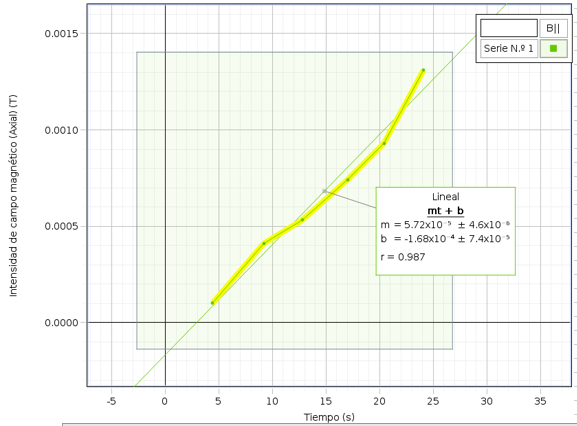
\includegraphics[scale=0.4]{../imgs/a.png}
   \caption{Corriente vs tiempo}
   \label{Fig:1}
\end{figure}

En la gráfica de la figura \ref{Fig:1}
se puede apreciar una línea ascendente, siendo esta la gráfica en la que se registraron los aumentos de la corriente en la bobina, resultando en la recta mostrada en la gráfica 1.
Igualmente, la perfección de la recta de acuerdo con los valores obtenidos fue de un 98\%, siendo una medición bastante buena debido a la exactitud de la misma.

\begin{figure}[H]
   \centering
   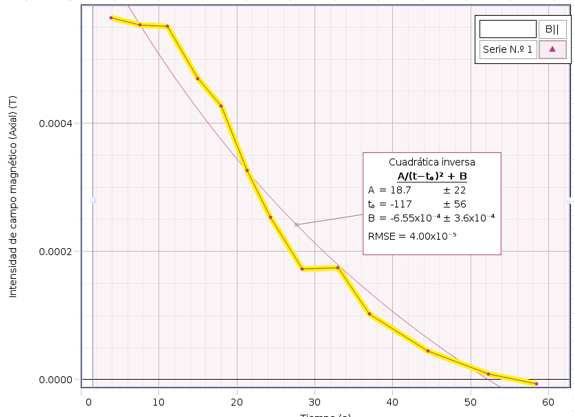
\includegraphics[scale=0.4]{../imgs/a1.png}
   \caption{Corriente vs tiempo}
   \label{Fig:2}
\end{figure}


\begin{figure}[H]
   \centering
   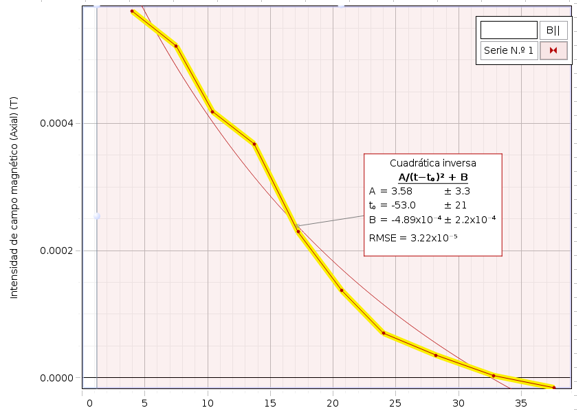
\includegraphics[scale=0.4]{../imgs/a2.png}
   \caption{Corriente vs tiempo}
   \label{Fig:3}
\end{figure}


\begin{figure}[H]
   \centering
   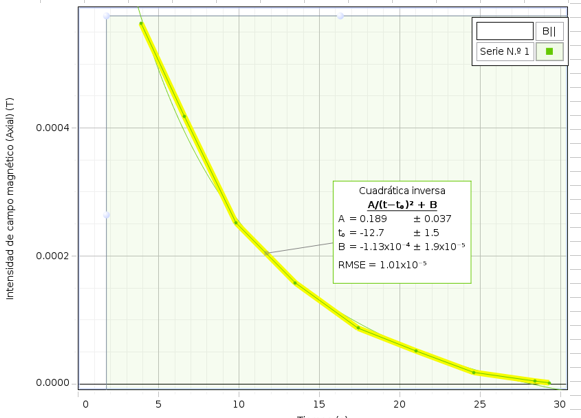
\includegraphics[scale=0.4]{../imgs/a3.png}
   \caption{Corriente vs tiempo}
   \label{Fig:4}
\end{figure}


\begin{figure}[H]
   \centering
   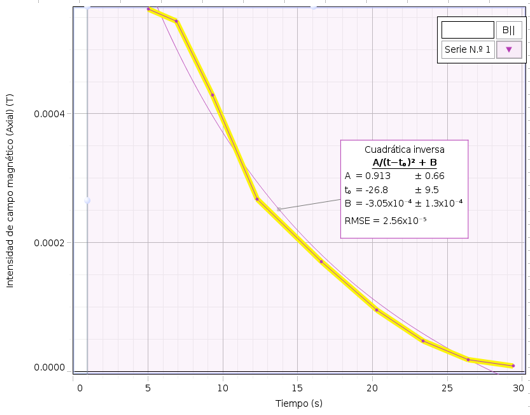
\includegraphics[scale=0.4]{../imgs/a4.png}
   \caption{Corriente vs tiempo}
   \label{Fig:5}
\end{figure}

\begin{figure}[H]
   \centering
   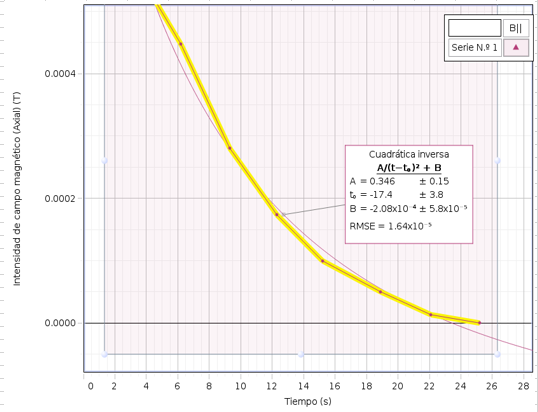
\includegraphics[scale=0.4]{../imgs/a5.png}
   \caption{Corriente vs tiempo}
   \label{Fig:6}
\end{figure}

En el resto de gráficas de las figuras \ref{Fig:2}, \ref{Fig:3}, \ref{Fig:4}, \ref{Fig:5} \& \ref{Fig:6} se registraron los valores de la intensidad de campo eléctrico obtenidos al ir alejando progresivamente la bobina del sensor, disminuyendo la intensidad del campo eléctrico medido por el sensor. Es por ello que la gráfica va progresando de manera descendente. 

\subsection*{Comportamiento del campo magnético en la dirección axial}

El comportamiento del campo magnético en la dirección axial, es decir, a lo largo del eje de un imán o en relación con una bobina solenoide, depende de la configuración de las fuentes magnéticas y de la ubicación del punto de interés en relación con esas fuentes. En un solenoide, que es una bobina enrollada de alambre con corriente eléctrica, el campo magnético en la dirección axial es generalmente uniforme y se asemeja al campo de un imán ideal. Las líneas del campo magnético en un solenoide fluyen desde un extremo al otro de la bobina.

\begin{itemize}
\item Dentro del solenoide: En la dirección axial del solenoide, el campo magnético es esencialmente constante y uniforme. Las líneas de campo magnético son paralelas al eje del solenoide y apuntan en la misma dirección.
\item Fuera del solenoide: Fuera del solenoide, el campo magnético se debilita rápidamente y tiende a aproximarse a cero en distancias significativas del solenoide.
\end{itemize}

De acuerdo a lo investigado, el experimento se asemeja bastante al comportamiento ideal del campo magnético en la dirección axial para un solenoide, debido a que las gráficas registradas son casi uniformes, tal y como lo explica la teoría que deberían de ser las líneas del campo magnético.


\section{Conclusiones}\label{Conclusiones}				% -------------------- Conclusiones
El objetivo si se cumplió, la teoría se asemejo muy bien a la práctica y como se pudo observar en las gráficas y como ya mencionado el comportamiento de nuestros datos es el correcto, por otro lado
y regresando a la teoría, la fuerza magnética es un componente fundamental del universo físico y continúa siendo un área activa de investigación en la física. A medida que continuamos explorando y comprendiendo mejor esta fuerza, es probable que descubramos aún más aplicaciones y fenómenos fascinantes relacionados con el magnetismo. 

\begin{thebibliography}{9}						% -------------------- Bibliografía
	\bibitem{Porto}
 Porto, J. P., \& Merino, M. (2021, 2 agosto). Fuerza magnética - qué es, definición y concepto. Definición.de. https://definicion.de/fuerza-magnetica/
	\bibitem{Serway}
	Serway, R. A., $\&$ Jewett, J. W. (2008). Física para ciencias e ingeniería. (7.a
ed., Vol. 1). CENGAGE Learning.

\bibitem{Pérez}
	Newton, I. (1687). Philosophiæ Naturalis Principia Mathematica [Mathematical Principles of Natural Philosophy]. Londini: Jussu Societatis Regiæ ac Typis Josephi Streater.

\end{thebibliography}
\end{document}	